In this appendix, we present all testing results for the scenarios described in the main text. The results for each testing case are similar to those presented in Section \ref{sec:c1-results}; however, the reader may find it helpful to review the measurements for other test cases. Figures \ref{fig:c2-clutter}, \ref{fig:c3-clutter}, and \ref{fig:c4-clutter} show the change of metrics depending on the change of the clutter spatial rate $\lambda_c$ for scenarios (C2), (C3), and (C4), respectively. Figures \ref{fig:c2-pd}, \ref{fig:c3-pd}, and \ref{fig:c4-pd} depict the change of metrics for different values of the detection probability $P_{D,k}$ for each individual case in the same order. Figures \ref{fig:c2-ps}, \ref{fig:c3-ps}, and \ref{fig:c4-ps} show the change for the survival probability $P_{S,k}$, Figures \ref{fig:c2-tau}, \ref{fig:c3-tau}, and \ref{fig:c4-tau} for the truncation threshold $\tau$, and finally, Figures \ref{fig:c2-u}, \ref{fig:c3-u}, and \ref{fig:c4-u} for the merge threshold $U$ for scenarios (C2), (C3), and (C4), respectively. All figures are ordered in a way in which metrics for one parameter are grouped together so that the reader can compare results for different test cases. Every figure is provided with a detailed description of what it depicts.

\newpage  % three figures per page, otherwise one is placed under the par above

%%%%%%%%%%%%%%%%%%%%%%%%%%%%%%%%%%%%%%%%%%%%%%%%
% Clutter rate
%%%%%%%%%%%%%%%%%%%%%%%%%%%%%%%%%%%%%%%%%%%%%%%%

\begin{figure}
    \centering
    \begin{subfigure}[]{0.48\linewidth}
        \centering
        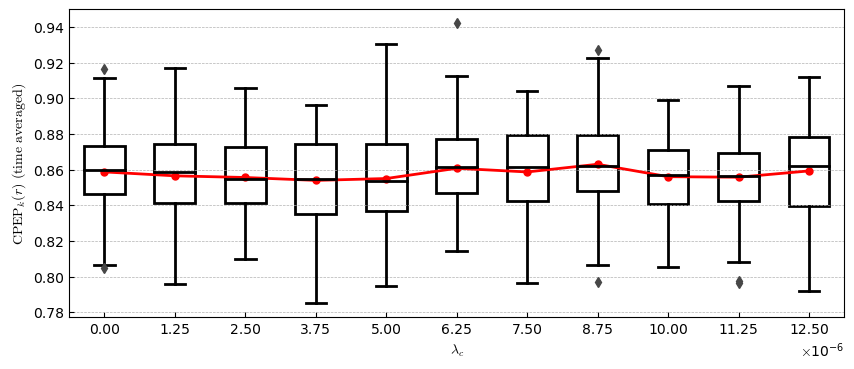
\includegraphics[width=\linewidth]{figures/c2-clutter-cpep.png}
    \end{subfigure}
    \hfill
    \begin{subfigure}[]{0.48\linewidth}
        \centering
        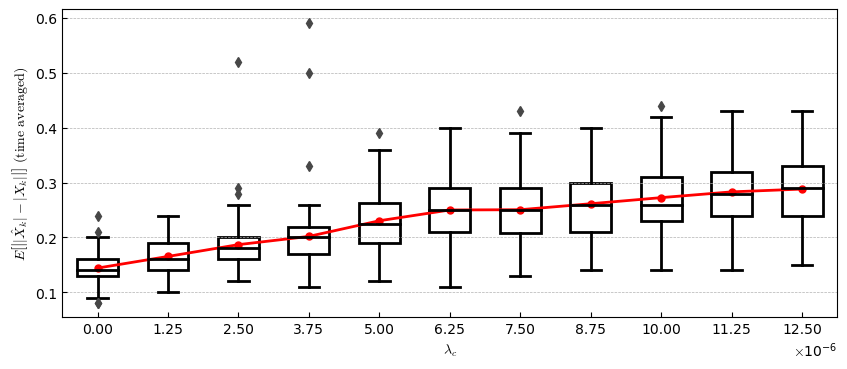
\includegraphics[width=\linewidth]{figures/c2-clutter-eae.png}
    \end{subfigure}
  \caption[(C2). Change of performance depending on the clutter rate.]{Here, we examine the change of CPEP (left) and the expected absolute error on the number of targets (right) for the (C2) scenario for different values of the clutter spatial rate $\lambda_c$. Every box is the representation of the distribution of $100$ independent samples. As the clutter spatial rate increases, the estimation error also increases, which may be observed on the growing trend of both metrics. All other setting are set to default values, i.e. $P_{D,k} = 0.98$, $P_{S,k} = 0.99$, $\tau = 10^{-5}$ and $U = 4$.}
  \label{fig:c2-clutter}
\end{figure}

\begin{figure}
    \centering
    \begin{subfigure}[]{0.48\linewidth}
        \centering
        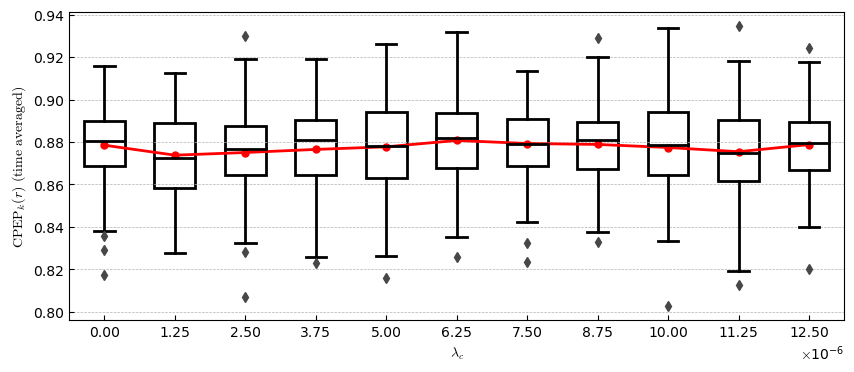
\includegraphics[width=\linewidth]{figures/c3-clutter-cpep.png}
    \end{subfigure}
    \hfill
    \begin{subfigure}[]{0.48\linewidth}
        \centering
        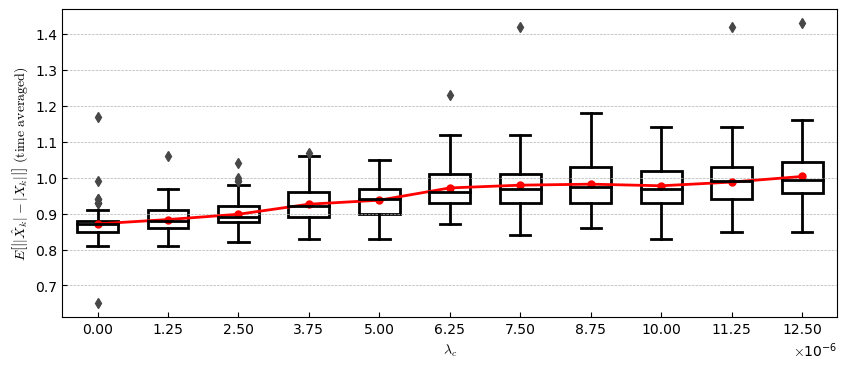
\includegraphics[width=\linewidth]{figures/c3-clutter-eae.png}
    \end{subfigure}
  \caption[(C3). Change of performance depending on the clutter rate.]{Here, we examine the change of CPEP (left) and the expected absolute error on the number of targets (right) for the (C3) scenario for different values of the clutter spatial rate $\lambda_c$. Every box is the representation of the distribution of $100$ independent samples. As the clutter spatial rate increases, the estimation error also increases, which may be observed on the growing trend of both metrics. All other setting are set to default values, i.e. $P_{D,k} = 0.98$, $P_{S,k} = 0.99$, $\tau = 10^{-5}$ and $U = 4$.}
  \label{fig:c3-clutter}
\end{figure}

\begin{figure}
    \centering
    \begin{subfigure}[]{0.48\linewidth}
        \centering
        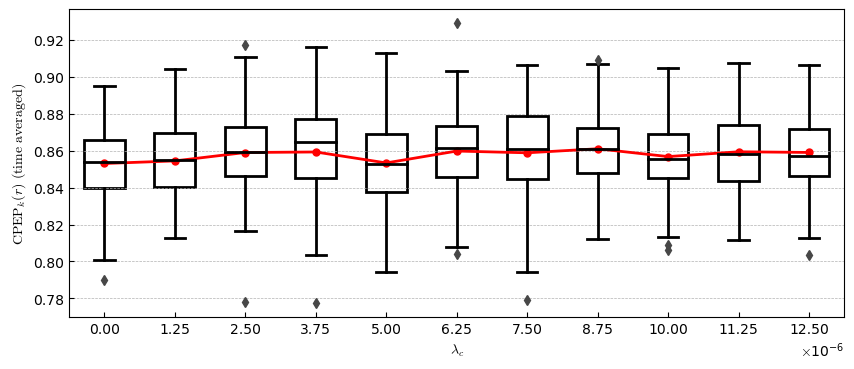
\includegraphics[width=\linewidth]{figures/c4-clutter-cpep.png}
    \end{subfigure}
    \hfill
    \begin{subfigure}[]{0.48\linewidth}
        \centering
        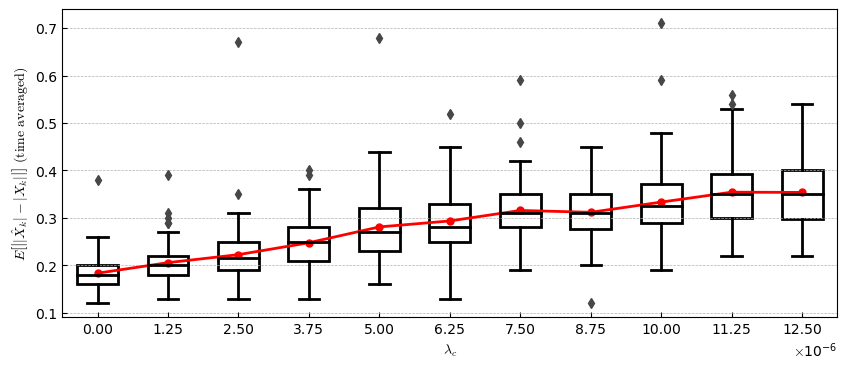
\includegraphics[width=\linewidth]{figures/c4-clutter-eae.png}
    \end{subfigure}
  \caption[(C4). Change of performance depending on the clutter rate.]{Here, we examine the change of CPEP (left) and the expected absolute error on the number of targets (right) for the (C4) scenario for different values of the clutter spatial rate $\lambda_c$. Every box is the representation of the distribution of $100$ independent samples. As the clutter spatial rate increases, the estimation error also increases, which may be observed on the growing trend of both metrics. All other setting are set to default values, i.e. $P_{D,k} = 0.98$, $P_{S,k} = 0.99$, $\tau = 10^{-5}$ and $U = 4$.}
  \label{fig:c4-clutter}
\end{figure}

%%%%%%%%%%%%%%%%%%%%%%%%%%%%%%%%%%%%%%%%%%%%%%%%
% Probability of detection
%%%%%%%%%%%%%%%%%%%%%%%%%%%%%%%%%%%%%%%%%%%%%%%%

\begin{figure}
    \centering
    \begin{subfigure}[]{0.48\linewidth}
        \centering
        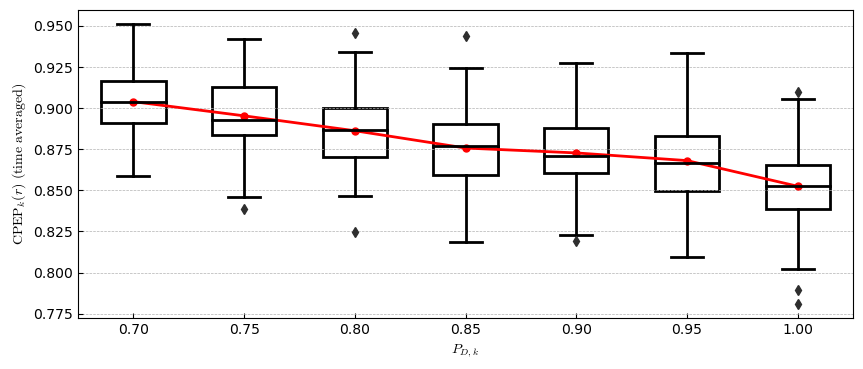
\includegraphics[width=\linewidth]{figures/c2-pd-cpep.png}
    \end{subfigure}
    \hfill
    \begin{subfigure}[]{0.48\linewidth}
        \centering
        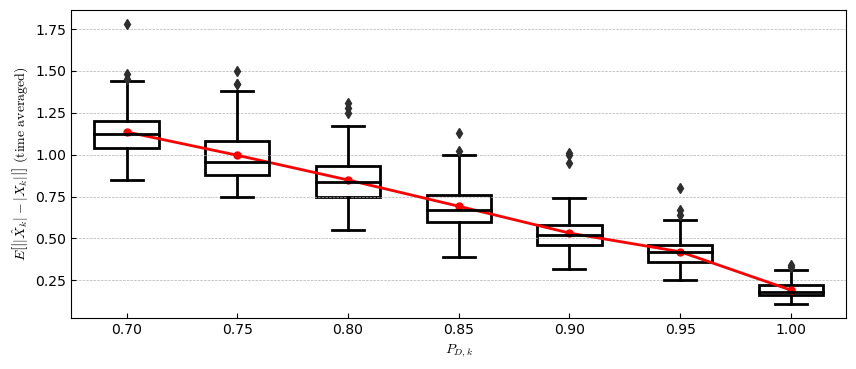
\includegraphics[width=\linewidth]{figures/c2-pd-eae.png}
    \end{subfigure}
  \caption[(C2). Change of performance depending on the detection probability.]{The change of CPEP (left) and the expected absolute error on the number of targets (right) for the (C2) scenario for different values of the detection probability $P_{D,k}$. Every box is the representation of the distribution of $100$ independent samples. As the detection probability increases, the estimation error decreases, which may be observed on the decreasing trend of both metrics. All other setting are set to default values, i.e. $\lambda_{c} = 12.5 \times 10^{-6}$, $P_{S,k} = 0.99$, $\tau = 10^{-5}$ and $U = 4$.}
  \label{fig:c2-pd}
\end{figure}

\begin{figure}
    \centering
    \begin{subfigure}[]{0.48\linewidth}
        \centering
        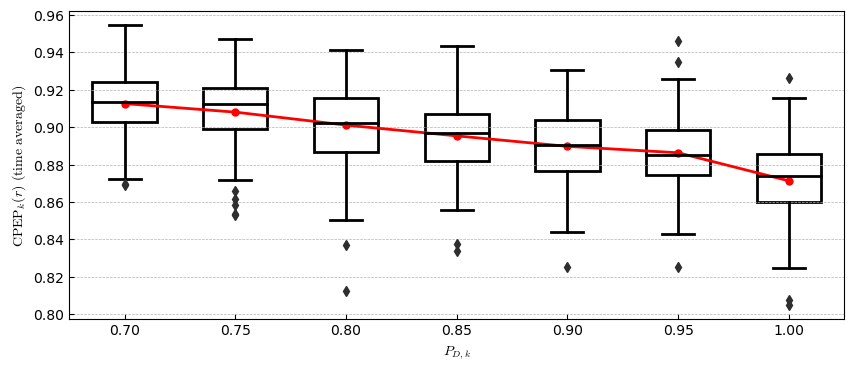
\includegraphics[width=\linewidth]{figures/c3-pd-cpep.png}
    \end{subfigure}
    \hfill
    \begin{subfigure}[]{0.48\linewidth}
        \centering
        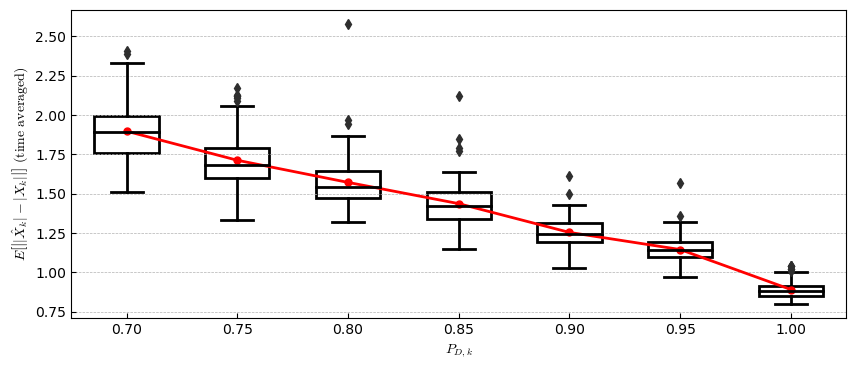
\includegraphics[width=\linewidth]{figures/c3-pd-eae.png}
    \end{subfigure}
  \caption[(C3). Change of performance depending on the detection probability.]{The change of CPEP (left) and the expected absolute error on the number of targets (right) for the (C3) scenario for different values of the detection probability $P_{D,k}$. Every box is the representation of the distribution of $100$ independent samples. As the detection probability increases, the estimation error decreases, which may be observed on the decreasing trend of both metrics. All other setting are set to default values, i.e. $\lambda_{c} = 12.5 \times 10^{-6}$, $P_{S,k} = 0.99$, $\tau = 10^{-5}$ and $U = 4$.}
  \label{fig:c3-pd}
\end{figure}

\begin{figure}
    \centering
    \begin{subfigure}[]{0.48\linewidth}
        \centering
        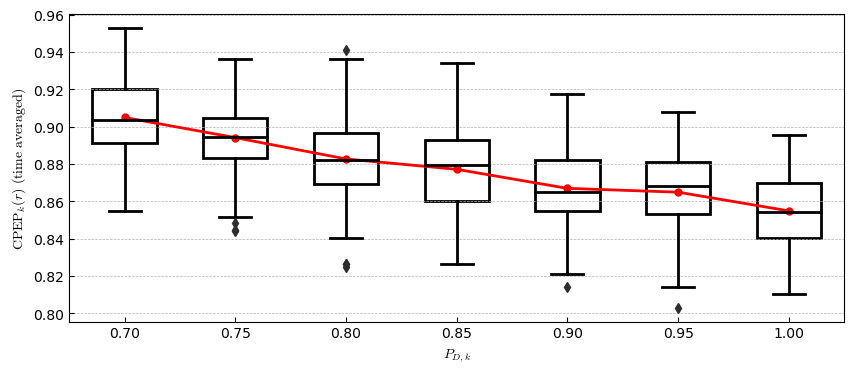
\includegraphics[width=\linewidth]{figures/c4-pd-cpep.png}
    \end{subfigure}
    \hfill
    \begin{subfigure}[]{0.48\linewidth}
        \centering
        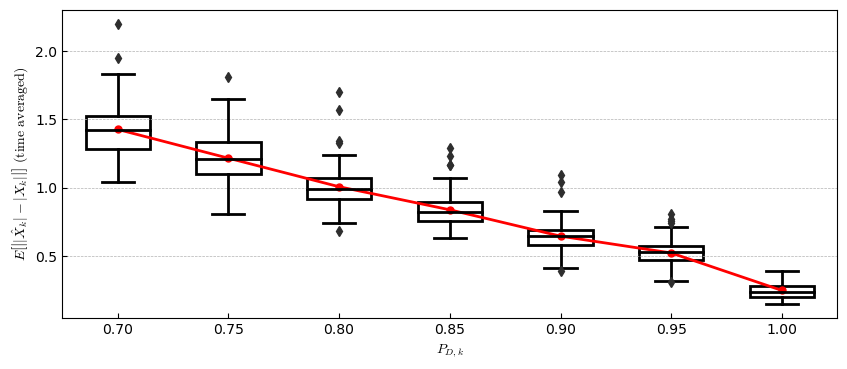
\includegraphics[width=\linewidth]{figures/c4-pd-eae.png}
    \end{subfigure}
  \caption[(C4). Change of performance depending on the detection probability.]{The change of CPEP (left) and the expected absolute error on the number of targets (right) for the (C4) scenario for different values of the detection probability $P_{D,k}$. Every box is the representation of the distribution of $100$ independent samples. As the detection probability increases, the estimation error decreases, which may be observed on the decreasing trend of both metrics. All other setting are set to default values, i.e. $\lambda_{c} = 12.5 \times 10^{-6}$, $P_{S,k} = 0.99$, $\tau = 10^{-5}$ and $U = 4$.}
  \label{fig:c4-pd}
\end{figure}

%%%%%%%%%%%%%%%%%%%%%%%%%%%%%%%%%%%%%%%%%%%%%%%%
% Probability of survival
%%%%%%%%%%%%%%%%%%%%%%%%%%%%%%%%%%%%%%%%%%%%%%%%

\begin{figure}
    \centering
    \begin{subfigure}[]{0.48\linewidth}
        \centering
        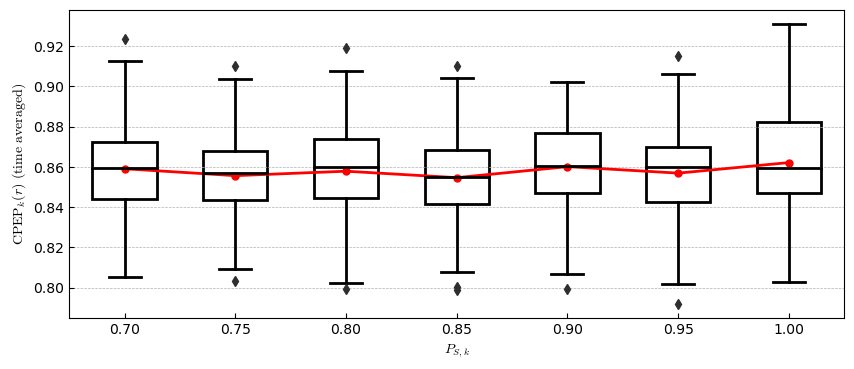
\includegraphics[width=\linewidth]{figures/c2-ps-cpep.png}
    \end{subfigure}
    \hfill
    \begin{subfigure}[]{0.48\linewidth}
        \centering
        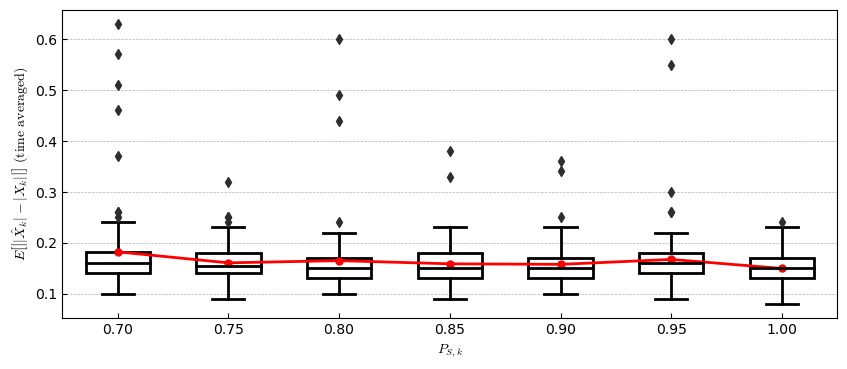
\includegraphics[width=\linewidth]{figures/c2-ps-eae.png}
    \end{subfigure}
  \caption[(C2). Change of performance depending on the survival probability.]{The change of CPEP (left) and the expected absolute error on the number of targets (right) for the (C2) scenario for different values of the survival probability $P_{S,k}$. Every box is the representation of the distribution of $100$ independent samples. Neither of metrics shows a change when the survival probability changes. All other setting are set to default values, i.e. $\lambda_{c} = 12.5 \times 10^{-6}$, $P_{D,k} = 0.98$, $\tau = 10^{-5}$ and $U = 4$.}
  \label{fig:c2-ps}
\end{figure}

\begin{figure}
    \centering
    \begin{subfigure}[]{0.48\linewidth}
        \centering
        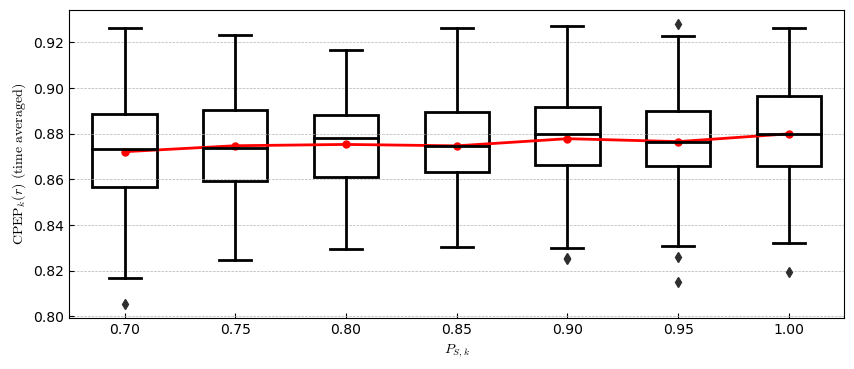
\includegraphics[width=\linewidth]{figures/c3-ps-cpep.png}
    \end{subfigure}
    \hfill
    \begin{subfigure}[]{0.48\linewidth}
        \centering
        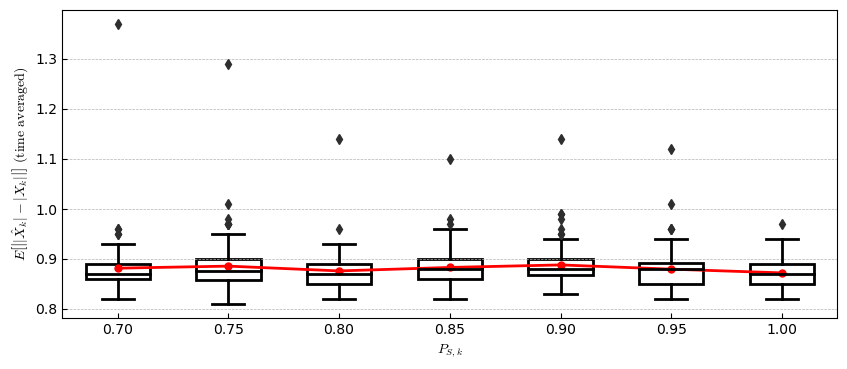
\includegraphics[width=\linewidth]{figures/c3-ps-eae.png}
    \end{subfigure}
  \caption[(C3). Change of performance depending on the survival probability.]{The change of CPEP (left) and the expected absolute error on the number of targets (right) for the (C3) scenario for different values of the survival probability $P_{S,k}$. Every box is the representation of the distribution of $100$ independent samples. Neither of metrics shows a change when the survival probability changes. All other setting are set to default values, i.e. $\lambda_{c} = 12.5 \times 10^{-6}$, $P_{D,k} = 0.98$, $\tau = 10^{-5}$ and $U = 4$.}
  \label{fig:c3-ps}
\end{figure}

\begin{figure}
    \centering
    \begin{subfigure}[]{0.48\linewidth}
        \centering
        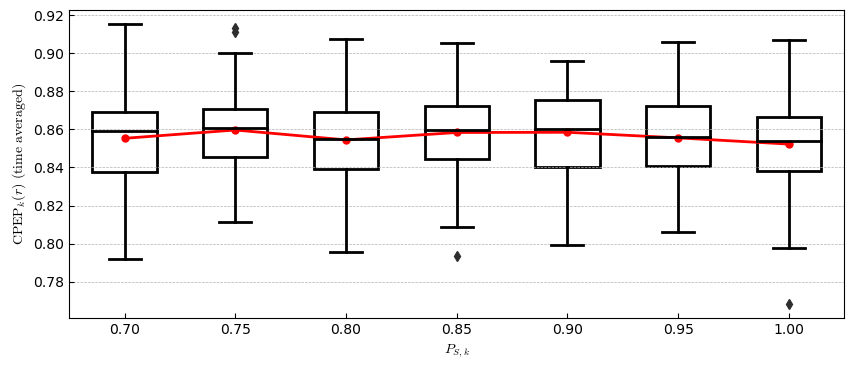
\includegraphics[width=\linewidth]{figures/c4-ps-cpep.png}
    \end{subfigure}
    \hfill
    \begin{subfigure}[]{0.48\linewidth}
        \centering
        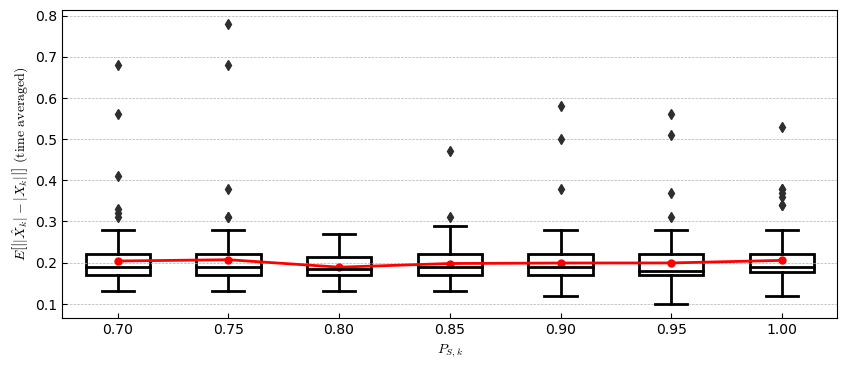
\includegraphics[width=\linewidth]{figures/c4-ps-eae.png}
    \end{subfigure}
  \caption[(C4). Change of performance depending on the survival probability.]{The change of CPEP (left) and the expected absolute error on the number of targets (right) for the (C4) scenario for different values of the survival probability $P_{S,k}$. Every box is the representation of the distribution of $100$ independent samples. Neither of metrics shows a change when the survival probability changes. All other setting are set to default values, i.e. $\lambda_{c} = 12.5 \times 10^{-6}$, $P_{D,k} = 0.98$, $\tau = 10^{-5}$ and $U = 4$.}
  \label{fig:c4-ps}
\end{figure}

%%%%%%%%%%%%%%%%%%%%%%%%%%%%%%%%%%%%%%%%%%%%%%%%
% Truncation threshold
%%%%%%%%%%%%%%%%%%%%%%%%%%%%%%%%%%%%%%%%%%%%%%%%

\begin{figure}
    \centering
    \begin{subfigure}[]{0.48\linewidth}
        \centering
        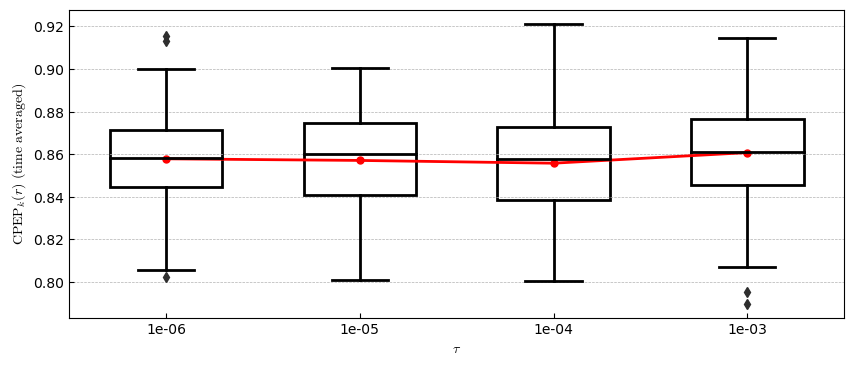
\includegraphics[width=\linewidth]{figures/c2-tau-cpep.png}
    \end{subfigure}
    \hfill
    \begin{subfigure}[]{0.48\linewidth}
        \centering
        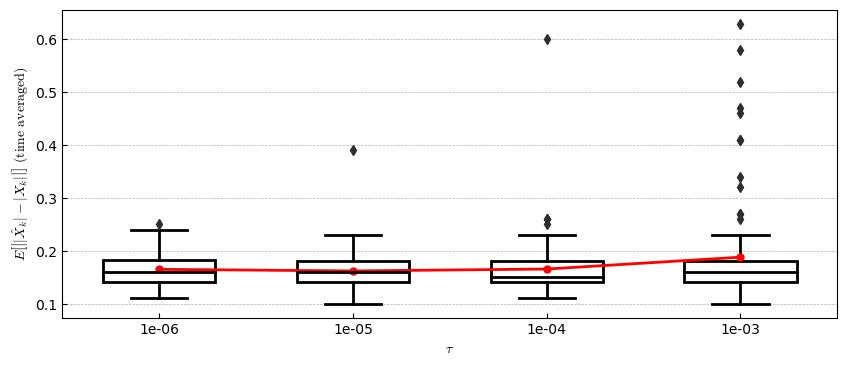
\includegraphics[width=\linewidth]{figures/c2-tau-eae.png}
    \end{subfigure}
  \caption[(C2). Change of performance depending on the prune threshold.]{The change of CPEP (left) and the expected absolute error on the number of targets (right) for the (C2) scenario for different values of the truncation threshold $\tau$. Every box is the representation of the distribution of $100$ independent samples. The X axis is on the logarithmic scale. We see, that, for higher values of $\tau$, the performance becomes worse. All other setting are set to default values, i.e. $\lambda_{c} = 12.5 \times 10^{-6}$, $P_{D,k} = 0.98$, $P_{S,k} = 0.99$ and $U = 4$.}
  \label{fig:c2-tau}
\end{figure}

\begin{figure}
    \centering
    \begin{subfigure}[]{0.48\linewidth}
        \centering
        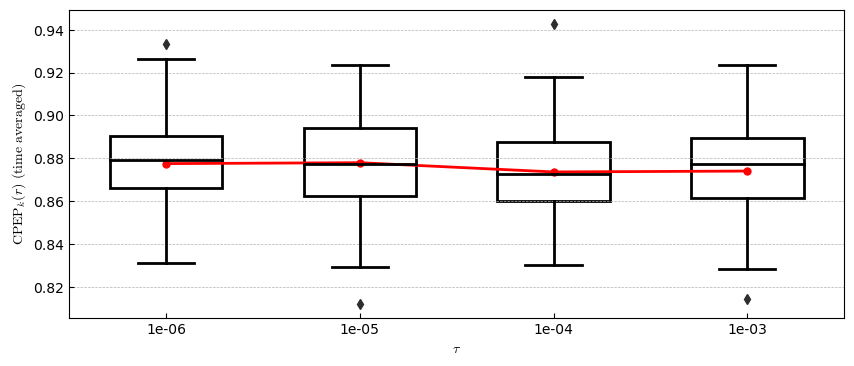
\includegraphics[width=\linewidth]{figures/c3-tau-cpep.png}
    \end{subfigure}
    \hfill
    \begin{subfigure}[]{0.48\linewidth}
        \centering
        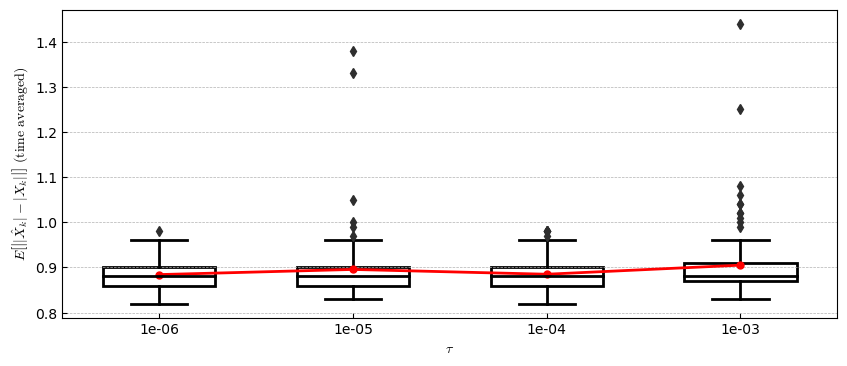
\includegraphics[width=\linewidth]{figures/c3-tau-eae.png}
    \end{subfigure}
  \caption[(C3). Change of performance depending on the prune threshold.]{The change of CPEP (left) and the expected absolute error on the number of targets (right) for the (C3) scenario for different values of the truncation threshold $\tau$. Every box is the representation of the distribution of $100$ independent samples. The X axis is on the logarithmic scale. We see, that, for higher values of $\tau$, the performance becomes worse. All other setting are set to default values, i.e. $\lambda_{c} = 12.5 \times 10^{-6}$, $P_{D,k} = 0.98$, $P_{S,k} = 0.99$ and $U = 4$.}
  \label{fig:c3-tau}
\end{figure}

\begin{figure}
    \centering
    \begin{subfigure}[]{0.48\linewidth}
        \centering
        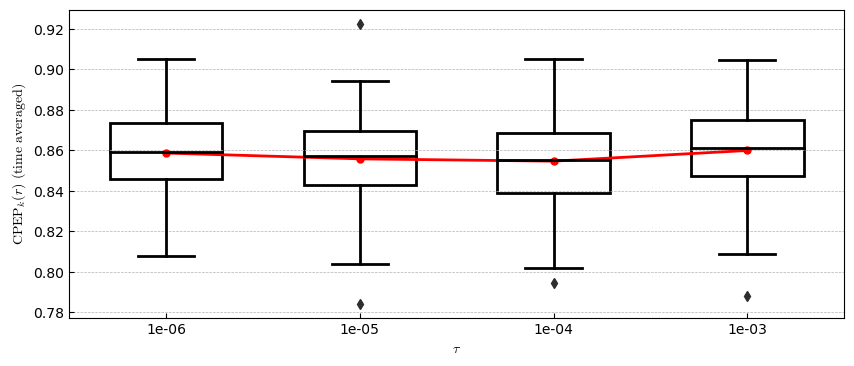
\includegraphics[width=\linewidth]{figures/c4-tau-cpep.png}
    \end{subfigure}
    \hfill
    \begin{subfigure}[]{0.48\linewidth}
        \centering
        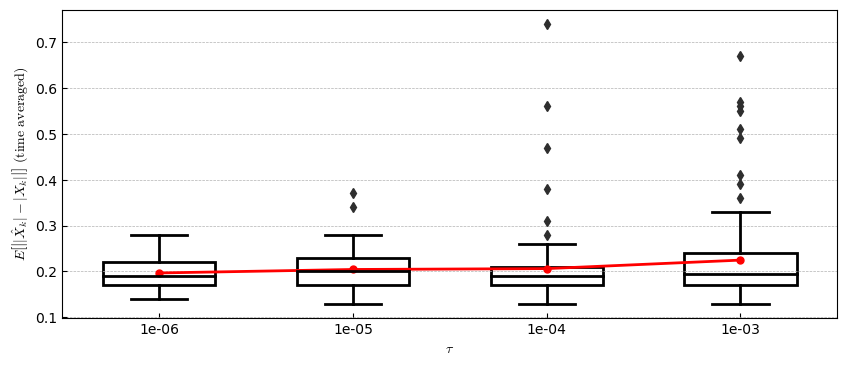
\includegraphics[width=\linewidth]{figures/c4-tau-eae.png}
    \end{subfigure}
  \caption[(C4). Change of performance depending on the prune threshold.]{The change of CPEP (left) and the expected absolute error on the number of targets (right) for the (C4) scenario for different values of the truncation threshold $\tau$. Every box is the representation of the distribution of $100$ independent samples. The X axis is on the logarithmic scale. We see, that, for higher values of $\tau$, the performance becomes worse. All other setting are set to default values, i.e. $\lambda_{c} = 12.5 \times 10^{-6}$, $P_{D,k} = 0.98$, $P_{S,k} = 0.99$ and $U = 4$.}
  \label{fig:c4-tau}
\end{figure}

%%%%%%%%%%%%%%%%%%%%%%%%%%%%%%%%%%%%%%%%%%%%%%%%
% Merge threshold
%%%%%%%%%%%%%%%%%%%%%%%%%%%%%%%%%%%%%%%%%%%%%%%%

\begin{figure}
    \centering
    \begin{subfigure}[]{0.48\linewidth}
        \centering
        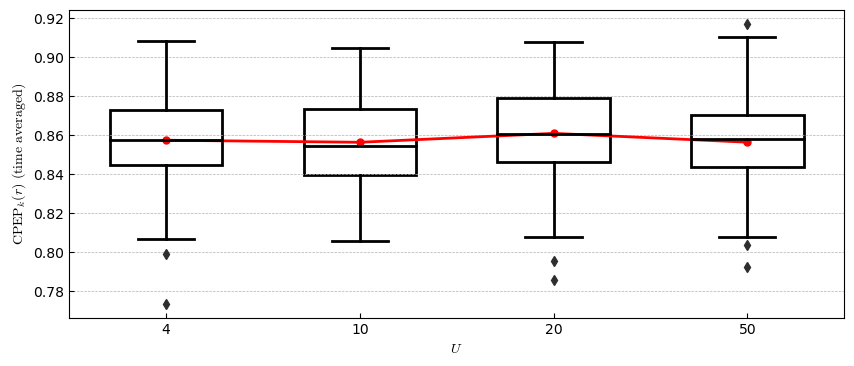
\includegraphics[width=\linewidth]{figures/c2-u-cpep.png}
    \end{subfigure}
    \hfill
    \begin{subfigure}[]{0.48\linewidth}
        \centering
        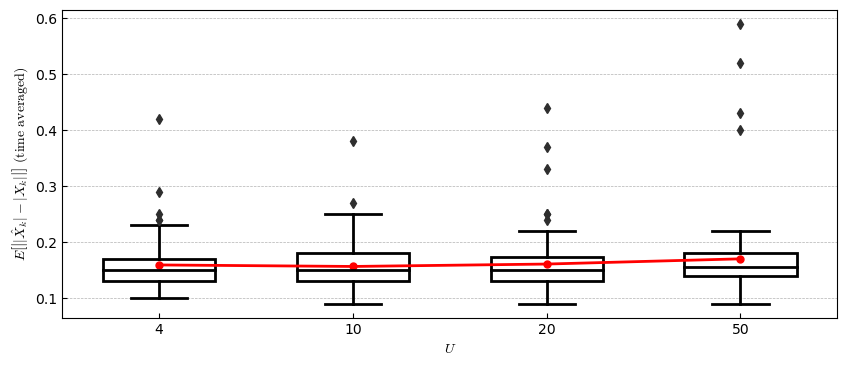
\includegraphics[width=\linewidth]{figures/c2-u-eae.png}
    \end{subfigure}
  \caption[(C2). Change of performance depending on the merge threshold.]{The change of CPEP (left) and the expected absolute error on the number of targets (right) for the (C2) scenario for different values of the merge threshold $U$. Every box is the representation of the distribution of $100$ independent samples. The X axis does not have any scale. We see that, for higher values of $U$, the performance slightly worsens. All other settings are set to default values, i.e. $\lambda_{c} = 12.5 \times 10^{-6}$, $P_{D,k} = 0.98$, $P_{S,k} = 0.99$, and $\tau = 10^{-5}$.}
  \label{fig:c2-u}
\end{figure}

\begin{figure}
    \centering
    \begin{subfigure}[]{0.48\linewidth}
        \centering
        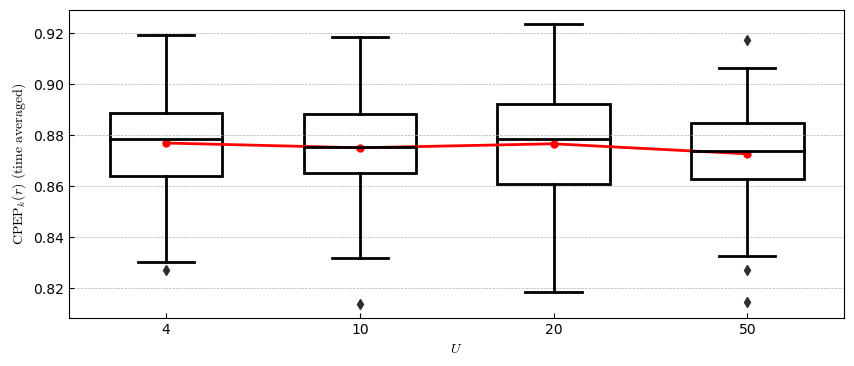
\includegraphics[width=\linewidth]{figures/c3-u-cpep.png}
    \end{subfigure}
    \hfill
    \begin{subfigure}[]{0.48\linewidth}
        \centering
        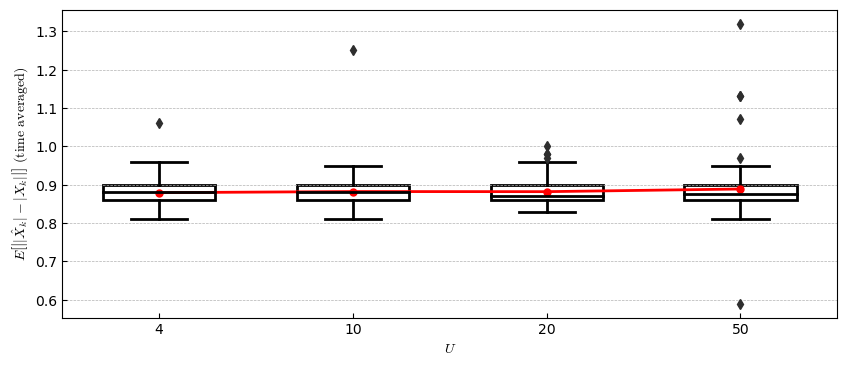
\includegraphics[width=\linewidth]{figures/c3-u-eae.png}
    \end{subfigure}
  \caption[(C3). Change of performance depending on the merge threshold.]{The change of CPEP (left) and the expected absolute error on the number of targets (right) for the (C3) scenario for different values of the merge threshold $U$. Every box is the representation of the distribution of $100$ independent samples. The X axis does not have any scale. We see that, for higher values of $U$, the performance slightly worsens. All other settings are set to default values, i.e. $\lambda_{c} = 12.5 \times 10^{-6}$, $P_{D,k} = 0.98$, $P_{S,k} = 0.99$, and $\tau = 10^{-5}$.}
  \label{fig:c3-u}
\end{figure}

\begin{figure}
    \centering
    \begin{subfigure}[]{0.48\linewidth}
        \centering
        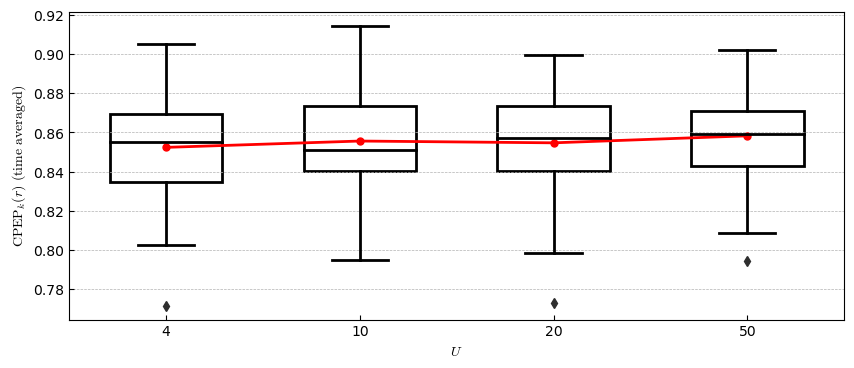
\includegraphics[width=\linewidth]{figures/c4-u-cpep.png}
    \end{subfigure}
    \hfill
    \begin{subfigure}[]{0.48\linewidth}
        \centering
        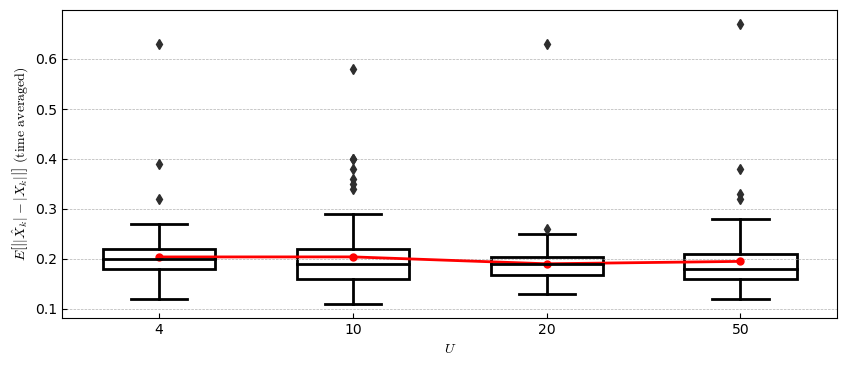
\includegraphics[width=\linewidth]{figures/c4-u-eae.png}
    \end{subfigure}
  \caption[(C4). Change of performance depending on the merge threshold.]{The change of CPEP (left) and the expected absolute error on the number of targets (right) for the (C4) scenario for different values of the merge threshold $U$. Every box is the representation of the distribution of $100$ independent samples. The X axis does not have any scale. We see that, for higher values of $U$, the performance slightly worsens. All other settings are set to default values, i.e. $\lambda_{c} = 12.5 \times 10^{-6}$, $P_{D,k} = 0.98$, $P_{S,k} = 0.99$, and $\tau = 10^{-5}$.}
  \label{fig:c4-u}
\end{figure}
